\chapter{\IfLanguageName{dutch}{Stand van zaken}{State of the art}}%
\label{ch:stand-van-zaken}

\section{Introductie}
Mendix vertegenwoordigt een van de toonaangevende low-code ontwikkelplatformen in het huidige softwareontwikkelingslandschap \autocite{Hermans2023}. Als implementatie van Model-Driven Development (MDD) principes stelt Mendix zowel professionele ontwikkelaars als zakelijke gebruikers in staat om applicaties te creëren via visuele modellering in plaats van traditionele codering. Het platform heeft aanzienlijke tractie gewonnen onder ondernemingen die hun digitale transformatie-initiatieven willen versnellen door ontwikkeltijd en technische complexiteit te verminderen \autocite{Oosten2020}.
\\
Hoewel Mendix via zijn modelgestuurde aanpak tal van voordelen biedt, waaronder verhoogde ontwikkelingssnelheid en bredere participatie van niet-technische belanghebbenden, presenteert het ook bepaalde beperkingen die de effectiviteit in verschillende contexten beïnvloeden \autocite{Yerukala2022}. Deze bachelorproef onderzoekt Mendix als een hedendaagse manifestatie van Model-Driven Development en analyseert kritisch de beperkingen ervan op het gebied van technische mogelijkheden, uitdagingen bij organisatorische adoptie en comparatieve nadelen ten opzichte van vergelijkbare platformen.
\\
Door zowel de theoretische onderbouwing van MDD als de praktische implementatie ervan in Mendix te begrijpen, beoogt dit onderzoek een uitgebreide beoordeling te geven van waar en hoe Mendix mogelijk tekortschiet in het aanpakken van complexe enterprise software behoeften, ondanks de innovatieve benadering van applicatieontwikkeling.
\newpage

\section{\IfLanguageName{dutch}{Model-Driven Development}{Model-Driven Development}}%
In dit hoofdstuk wordt de theoretische achtergrond van Model-Driven Development (MDD) en low-code ontwikkeling uiteengezet, met een specifieke focus op Mendix. Dit sluit aan bij de introductie van de stand van zaken, waarin het belang van MDD en low-code ontwikkeling werd geïntroduceerd. Dit hoofdstuk biedt een diepgaande analyse van MDD, inclusief de voordelen en beperkingen, en gaat na hoe Mendix binnen dit kader past.

\subsection{\IfLanguageName{dutch}{Kernconcepten van Model-Driven Development}{Core Concepts of Model-Driven Development}}%

Volgens het onderzoek \textcite{Hailpern2006} is MDD “een software engineering aanpak die bestaat uit de toepassing van modellen om het abstractieniveau te verhogen” in softwareontwikkeling. Deze aanpak ontstond als een natuurlijke evolutie in de overgang van low-level programmeertalen zoals assembly naar higher-level talen zoals Java en C\#, waarbij modellen de volgende stap in deze abstractie-evolutie vertegenwoordigen.

Het fundamentele principe achter MDD is dat het werken op hogere abstractieniveaus ontwikkelaars in staat stelt om complexe systemen effectiever en met minder inspanning te beheren. Dit komt overeen met de historische evolutie van programmeertalen, waarbij elke nieuwe generatie de abstractie vergrootte om de productiviteit te verbeteren en de cognitieve belasting van ontwikkelaars te verminderen.

\begin{figure}[H]
    \centering
    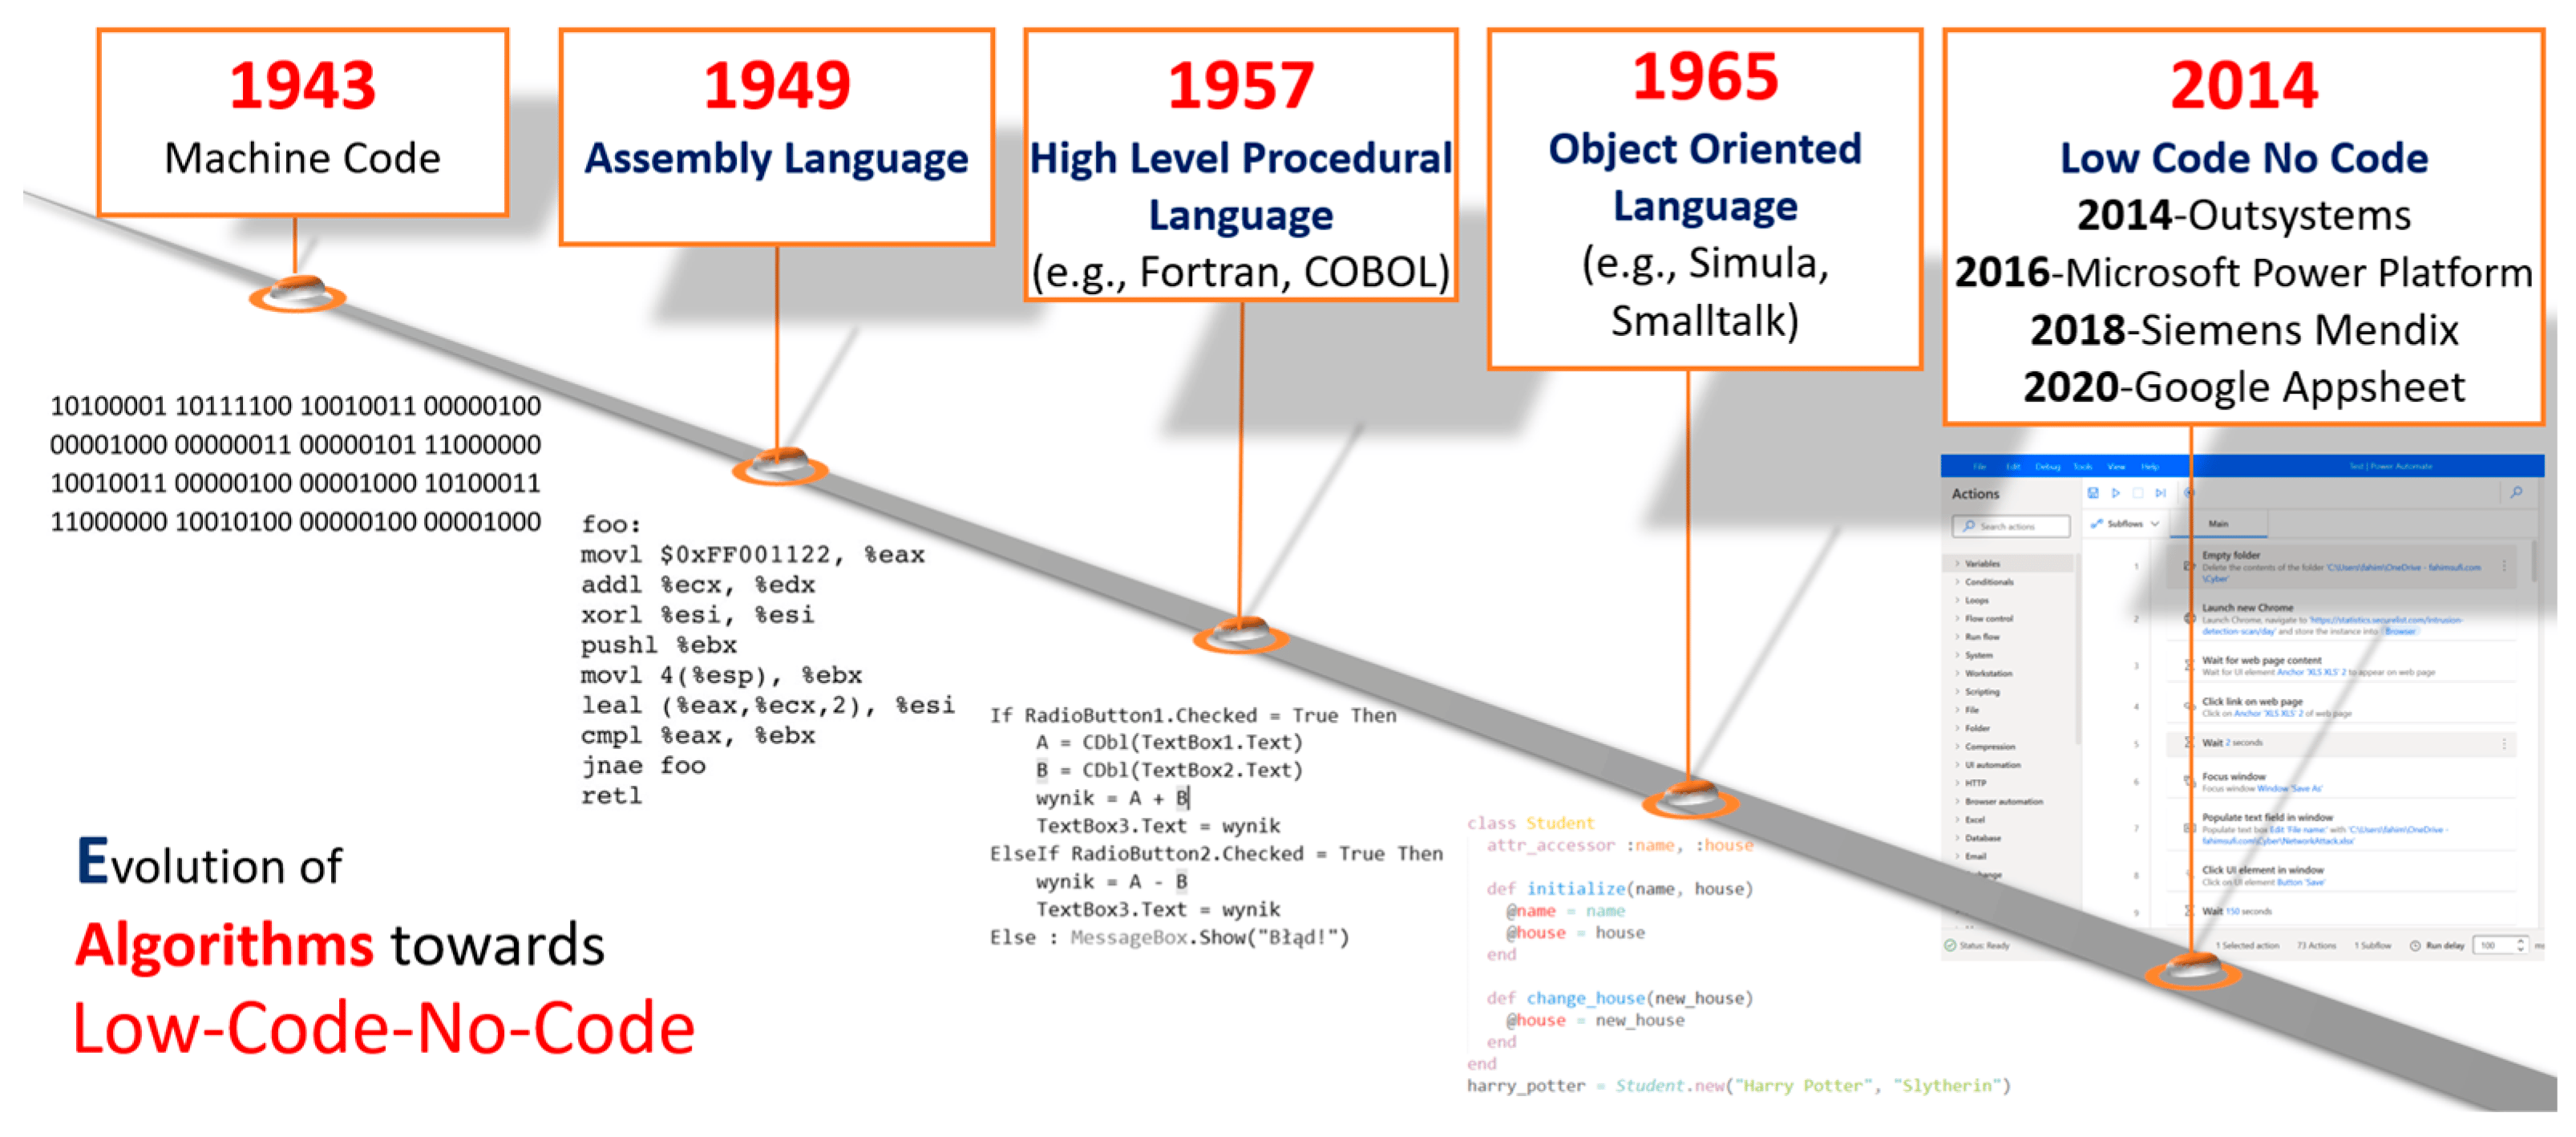
\includegraphics[width=0.8\textwidth]{Evolution_Of_Programming.jpg}
    \caption[Evolution]{\label{fig:evolution} Evolutie van programmeertalen naar steeds hogere abstractieniveau \autocite{Sufi_2023}.}
\end{figure}


\subsection{\IfLanguageName{dutch}{Historische context en evolutie}{Historical Context and Evolution}}%
Model Driven Development heeft een rijke geschiedenis die meer dan 20 jaar teruggaat \autocite{Henkel2010}. De evolutie verliep in verschillende fasen:

In de jaren '80 ontstonden de eerste geavanceerde modelleringsmethoden om de vereisten van informatiesystemen vast te leggen. Dit vormde de conceptuele basis voor MDD \autocite{Henkel2010}.

De jaren '90 brachten propriëtaire CASE-tools (Computer Aided Software Engineering), die informatiesystemen gedeeltelijk konden genereren op basis van modellen. Deze tools hadden echter beperkingen - vaak konden ze alleen codetemplates genereren waarna programmeurs de rest handmatig moesten aanvullen \autocite{Case_1985}.

Modernere benaderingen omvatten OMG's Model Driven Architecture (MDA) en executable UML (xUML). MDA werkt met verschillende modelleringsniveaus en transformaties tussen deze niveaus naar code, waarbij de gegenereerde code verder kan worden uitgewerkt \autocite{Soley2000}. xUML daarentegen streeft naar volledige codegeneratie zonder handmatige aanvullingen.

Er bestaan grote verschillen tussen oudere CASE-tools zoals Oracle Forms en Microsoft Access Forms en nieuwere tools gebaseerd op open standaarden zoals OptimalJ. Hoewel beide soorten tools MDD ondersteunen door abstractieniveaus te verhogen, bieden tools zoals OptimalJ meer controle over modeltransformaties en codegeneratie, terwijl formulier-gebaseerde tools zoals Oracle Forms minder controle bieden \autocite{Henkel2010}.

Ondanks deze verschillen delen alle MDD-benaderingen één fundamenteel doel: het verhogen van het abstractieniveau in softwareontwikkeling, waardoor ontwikkelaars complexere systemen kunnen bouwen met minder inspanning - vergelijkbaar met de evolutie van assembly-taal naar hogere programmeertalen zoals C\# en Java.


\subsection{\IfLanguageName{dutch}{Voordelen van Model-Driven Development}{Benefits of Model-Driven Development}}%
De literatuur identificeert verschillende belangrijke voordelen van het gebruik van MDD-benaderingen \autocite{Soley2000}. Door te werken met goed gedefinieerde modellen kunnen ontwikkelaars het aantal implementatiefouten verminderen, waardoor de softwarekwaliteit verbetert. Hogere abstractieniveaus stellen ontwikkelaars in staat om zich te richten op bedrijfslogica in plaats van technische implementatiedetails, wat de productiviteit van ontwikkelaars verhoogt. Modellen geven een duidelijker inzicht in de systeemstructuur en het gedrag, waardoor het ontwikkelproces beter onder controle is.

Bovendien vermindert het automatisch genereren van code de handmatige codeerinspanning en de bijbehorende fouten, wat leidt tot lagere ontwikkel- en onderhoudskosten. Snellere ontwikkelcycli helpen organisaties efficiënter om te gaan met hun applicatieontwikkelingsbehoeften, waardoor de ontwikkelingsachterstand afneemt. De mogelijkheid om snel iteraties uit te voeren en werkende functionaliteit te demonstreren verbetert de betrokkenheid van belanghebbenden, waardoor de klanttevredenheid toeneemt.

\subsection{\IfLanguageName{dutch}{Belangrijkste functionaliteitsgebieden voor MDD-tools}{Benefits of Model-Driven Development}}%
Om een MDD-tool effectief te laten zijn, moet het verschillende kritieke functionaliteiten ondersteunen, die kunnen worden gecategoriseerd in ondersteuning van zowel het modelleren als het ontwikkelproces.

Effectieve ondersteuning bij het modelleren vereist dat tools de juiste abstractieniveaus hanteren, waarbij irrelevante details worden verborgen terwijl essentiële concepten worden blootgelegd. 

Dit is vooral belangrijk omdat belanghebbenden modellen voor verschillende doeleinden gebruiken. Modellen moeten begrijpelijk zijn voor zowel technische als niet-technische belanghebbenden, idealiter met behulp van intuïtieve, voorspelbare notatie - veel tools maken om deze reden gebruik van UML, omdat dit wordt beschouwd als de de-facto standaard in de industrie \autocite{Marin2015} .Modellen moeten uitvoerbaar zijn, zelfs als ze incompleet zijn, zodat incrementele ontwikkeling mogelijk is en ontwikkelaars het gedrag van het systeem kunnen voorspellen door middel van experimenten of formele analyse. 

Volwassen MDD-tools ondersteunen de verfijning van modellen en transformaties tussen verschillende abstractieniveaus, waardoor aanpasbare model-naar-model en model-naar-code transformaties mogelijk zijn. Volgens \textcite{Marin2015} “moeten MDD-tools de uitvoering van modellen mogelijk maken, ook al zijn ze onvolledig, maar wel geldig”, wat modelcorrectie en -validatie in een vroeg stadium vergemakkelijkt.

Ondersteuning van het ontwikkelproces omvat een reeks functies. Tools moeten duidelijke feedback geven over fouten, idealiter door direct te wijzen naar de modelcomponenten die problemen veroorzaken, vergelijkbaar met hoe compilers problematische code markeren. 
Omdat software meestal door teams wordt ontwikkeld, moeten MDD-tools modelvergelijking, samenvoeging en versiebeheer ondersteunen. 

\textcite{Marin2015} benadrukken dat “versiebeheer van modellen absoluut noodzakelijk is om industriële samenwerkingsprojecten te beheren, waarbij verschillende leden van een ontwikkelteam aan hetzelfde model kunnen werken”.Effectieve tools moeten snel compileren en implementeren, met een bijzonder efficiënte afhandeling van incrementele wijzigingen.


MDD-tools moeten integreren met bestaande systemen en ontwikkelomgevingen, waardoor verbindingen met ERP-systemen, legacy applicaties en andere bedrijfsinfrastructuur mogelijk worden. Een van de belangrijkste voordelen van MDD is dat een breder scala aan mensen kan deelnemen aan de ontwikkeling, waaronder bedrijfskundigen met beperkte programmeervaardigheden. Tools moeten de definitie en het gebruik van herbruikbare componenten, patronen en best practices in projecten vergemakkelijken. 

Door deze functies op te nemen kunnen MDD-tools beter aansluiten op de behoeften van de industrie en de succesvolle toepassing van het MDD-paradigma in softwareontwikkelingsprojecten ondersteunen.

\subsection{\IfLanguageName{dutch}{De evolutie naar low-code platformen}{The Evolution Toward Low-Code Platforms}}%
Model-Driven Development (MDD) is de laatste jaren sterk geëvolueerd, vooral met de opkomst van low-code platformen zoals Mendix. Deze platforms vertegenwoordigen een verfijning van MDD-principes, waardoor ze toegankelijker worden voor ontwikkelaars met verschillende vaardigheidsniveaus, terwijl de kernvoordelen van modelgedreven benaderingen behouden blijven.

Zoals \textcite{Henkel2010} aantoonden in hun analyse van Mendix, proberen moderne MDD-tools een balans te vinden tussen abstractie en controle, waardoor ontwikkelaars op bedrijfsniveau kunnen redeneren terwijl ze toch voldoende controle houden over het systeemgedrag. Deze evolutie heeft MDD-principes toegankelijk gemaakt voor een breder publiek, waardoor softwareontwikkeling democratischer wordt dan alleen voor traditionele programmeerexperts. \textcite{Henkel2010} benadrukken dat “low-code platforms zoals Mendix met succes de kloof hebben overbrugd tussen abstractie op hoog niveau en technische implementatie, waardoor zowel zakelijke belanghebbenden als ontwikkelaars effectief kunnen samenwerken.”

Concluderend kan gesteld worden dat Model-Driven Development een significante vooruitgang betekent in software engineering methodologie, door modellen te verheffen van secundaire documentatie tot primaire ontwikkelartefacten. Door het abstractieniveau te verhogen stelt MDD ontwikkelaars in staat om complexiteit effectiever te managen, waardoor de productiviteit kan toenemen, de kwaliteit kan verbeteren en softwareontwikkeling toegankelijker wordt voor een breder scala aan belanghebbenden.De integratie van MDD-principes in low-code platforms heeft het bereik verder vergroot, waardoor het een krachtig hulpmiddel is geworden voor moderne softwareontwikkeling.

\section{\IfLanguageName{dutch}{Low-code platformen}{Low-code platforms}}%
In de volgende paragrafen zullen we de belangrijkste kenmerken, sterke punten en beperkingen van verschillende toonaangevende low-code ontwikkelplatformen onderzoeken en vergelijken, waaronder OutSystems, Joget DX en Mendix. Elk platform biedt unieke mogelijkheden en komt tegemoet aan verschillende organisatorische behoeften en use cases. Door hun benaderingen van visuele ontwikkeling, schaalbaarheid, inzetmogelijkheden, maatwerk en integratiemogelijkheden te onderzoeken, willen we een duidelijk inzicht geven in hoe deze platforms zich tot elkaar verhouden. Uiteindelijk zal deze vergelijking duidelijk maken waarom Mendix de meest uitgebreide en veelzijdige oplossing is, met de beste balans tussen flexibiliteit, schaalbaarheid en geavanceerde functies voor bedrijven die hun digitale transformatie willen versnellen.
\subsection{\IfLanguageName{dutch}{OutSystems}{OutSystems}}
OutSystems is een robuust low-code platform dat bekend staat om zijn visuele ontwikkelomgeving en mogelijkheden op enterprise-niveau. 

\begin{figure}[H]
    \centering
    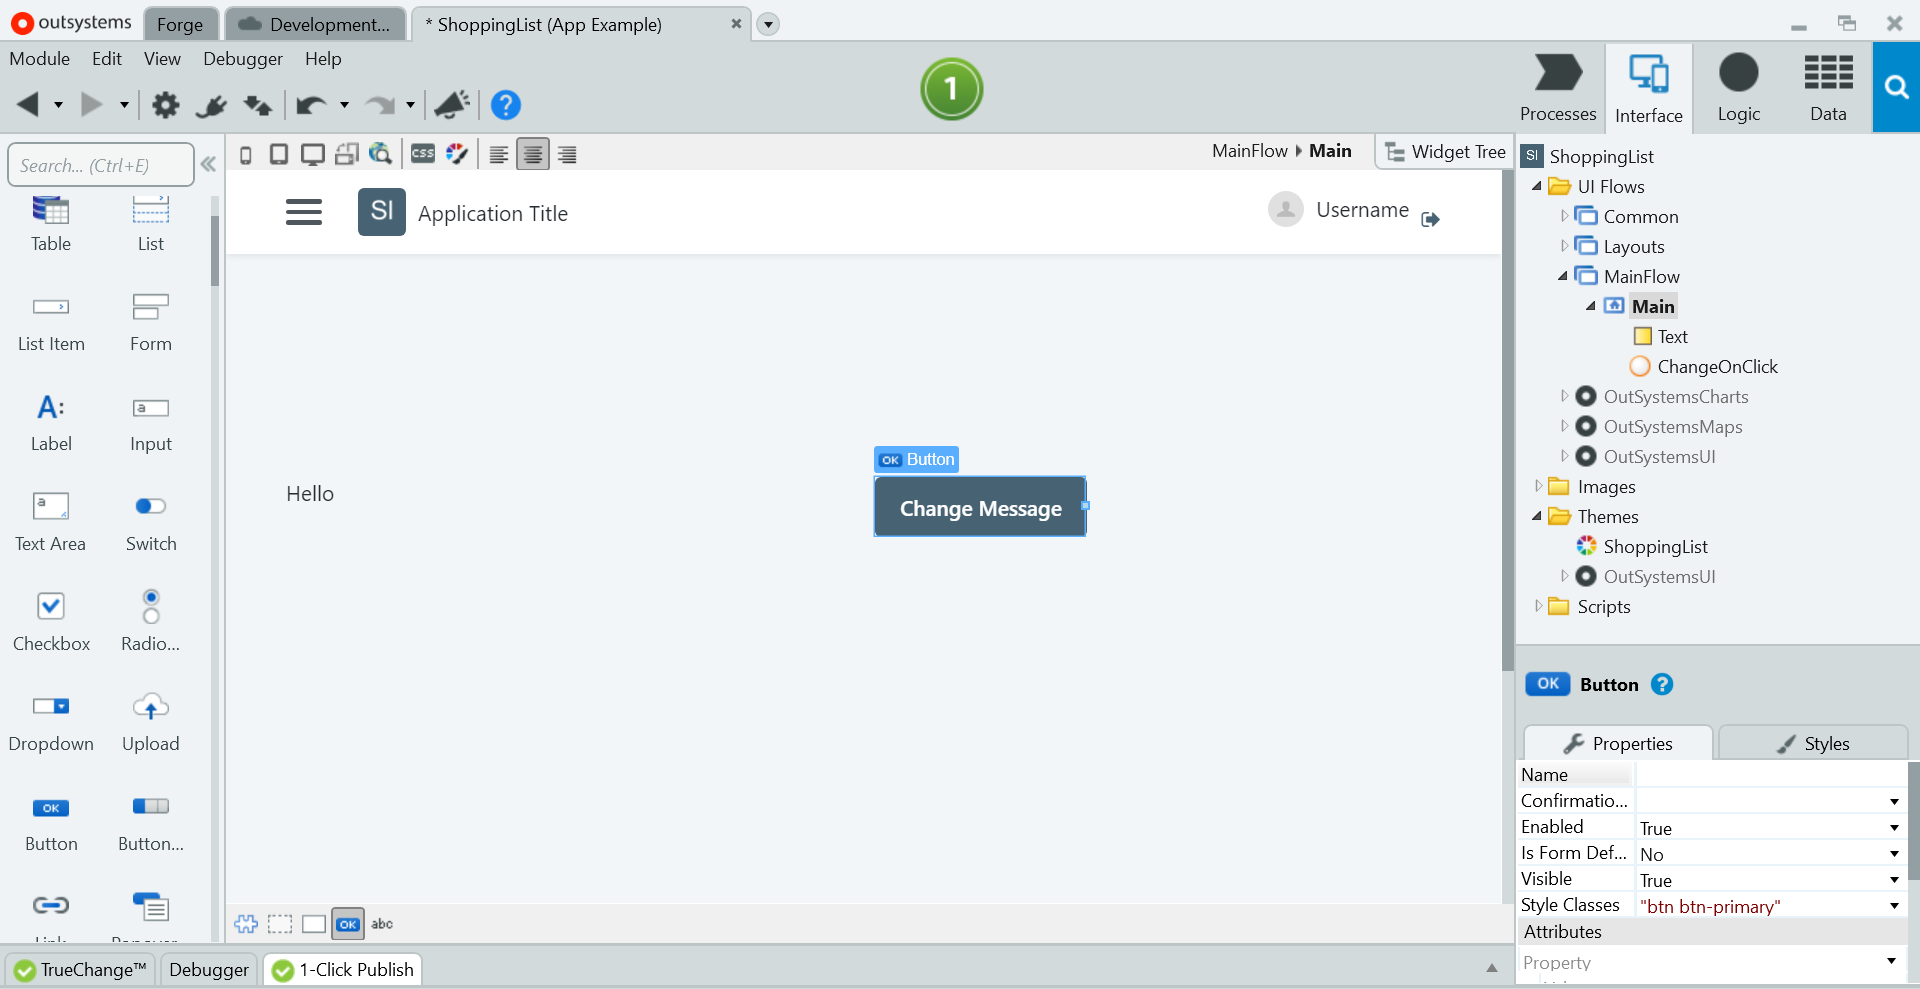
\includegraphics[width=0.8\textwidth]{OutSystems.png}
    \caption[Evolution]{\label{fig:outsystems} Visuele ontwikkelomgeving van OutSystems \autocite{FigueiraPutresza2021}.}
\end{figure}


Het blinkt uit in snelle applicatieontwikkeling en biedt zowel cloud-native als on-premises implementatieopties, die tegemoet komen aan uiteenlopende organisatorische behoeften \autocite{Sido2024}. OutSystems kan ook bogen op een levendig ecosysteem en community, samen met sterke beveiligingsfuncties en naleving van industriestandaarden. Het licentiemodel en de kostenbeperkingen kunnen echter onbetaalbaar zijn voor sommige organisaties, en de beperkte database-integratie en migratie-uitdagingen kunnen flexibiliteit in de weg staan \autocite{Sido2024}. Daarnaast kunnen de kwaliteit van de documentatie en de geïsoleerde ondersteuning van de community barrières opwerpen voor ontwikkelaars die het potentieel van het platform willen maximaliseren.
\subsection{\IfLanguageName{dutch}{Joget DX}{Joget DX}}
Joget DX daarentegen is een open-source platform dat de nadruk legt op eenvoud en snelle applicatieontwikkeling. Het is vooral sterk in de ontwikkeling van progressieve webapps (PWA's), gebruikerservaring (UX) en integratie met DevOps-praktijken \autocite{Sido2024}. Joget DX biedt ook uitbreidbaarheid via add-on builders en verbeterde workflowmogelijkheden, waardoor het een flexibele keuze is voor bedrijven die processen willen automatiseren. De beperkingen van het abonnementsmodel, de beperkte databasetoegang en de app-beperkingen kunnen de schaalbaarheid en aanpasbaarheid echter beperken \autocite{Sido2024}. Bovendien kunnen de leercurve en aanpassingscomplexiteit van het platform uitdagingen vormen voor gebruikers die overstappen van traditionele ontwikkelmethoden.
\subsection{\IfLanguageName{dutch}{Mendix}{Mendix}}
Mendix onderscheidt zich als het meest uitgebreide en veelzijdige low-code platform en biedt een breed scala aan functies voor zowel technische als niet-technische gebruikers. De modelgedreven ontwikkelaanpak, gecombineerd met microservices en containerisatie, zorgt voor schaalbaarheid, flexibiliteit en draagbaarheid. Mendix ondersteunt zowel cloud-native als on-premise infrastructuren en biedt daarmee flexibiliteit in de inzetmogelijkheden. Het volledige levenscyclusbeheer van het platform, de mogelijkheden voor kunstmatige intelligentie (AI) en machine learning (ML) en de functies voor procesautomatisering maken het een krachtig hulpmiddel voor ondernemingen \autocite{Sido2024}. Bovendien zorgen de openheid en uitbreidbaarheid van Mendix voor een naadloze integratie met externe systemen en aanpassingen om aan specifieke bedrijfsbehoeften te voldoen. Hoewel Mendix een aantal beperkingen heeft, zoals beperkte aanpasbaarheid van thema's en potentiële vendor lock-in, wegen de algehele mogelijkheden en het gebruiksgemak op tegen deze nadelen \autocite{Sido2024}.
\subsection{\IfLanguageName{dutch}{Keuze voor Mendix als low-code platform}{Choosing Mendix as low-code platform}}
Hoewel OutSystems en Joget DX waardevolle functies en mogelijkheden bieden, komt Mendix naar voren als het beste platform vanwege zijn uitgebreide en flexibele benadering van low-code ontwikkeling. Het vermogen om complexe bedrijfsapplicaties te ondersteunen, gecombineerd met de schaalbaarheid, uitbreidbaarheid en sterke focus op gebruikerservaring, maakt het de ideale keuze voor organisaties die op efficiënte en effectieve wijze digitale transformatie willen stimuleren.

\section{Mendix en high-code}
\subsection{Verschillende benaderingen}
Low-code en high-code representeren twee verschillende benaderingen van softwareontwikkeling, elk met unieke voordelen en uitdagingen. Low-code platforms, zoals Mendix, bieden een visuele ontwikkelomgeving waarin applicaties grotendeels zonder handmatig programmeren kunnen worden gebouwd \autocite{Krouwel_2022}. Dit versnelt de ontwikkeltijd en maakt softwareontwikkeling toegankelijker voor niet-technische gebruikers. Daarentegen biedt high-code, waarbij programmeertalen zoals Java of .NET worden gebruikt, maximale flexibiliteit en controle, wat essentieel is voor complexe of sterk aangepaste oplossingen \autocite{Krouwel_2022}. Hoewel low-code efficiënter is en snellere iteraties mogelijk maakt, kan het beperkingen hebben in maatwerk en prestaties vergeleken met high-code. De keuze tussen beide hangt af van de behoeften van de organisatie: low-code is ideaal voor snelle, aanpasbare applicaties, terwijl high-code de voorkeur geniet voor diepgaande technische en schaalbare oplossingen.

\subsection{Enterprise Flexibiliteit door Model-Based Engineering (MBE)}
\textcite{Krouwel_2022} benadrukt dat enterprise agility een cruciale succesfactor is in een steeds dynamischere markt, waarin bedrijven te maken hebben met hyperconcurrentie, veranderende regelgeving en technologische innovaties. Traditionele informatiesystemen vormen vaak een beperkende factor voor deze flexibiliteit, omdat ze hardcoded bedrijfsregels en structuren bevatten die moeilijk aanpasbaar zijn. Door Model-Based Engineering (MBE) te gebruiken, kunnen organisaties hun informatiesystemen ontwikkelen op basis van ontologische modellen, zoals die binnen de DEMO-methodologie worden gehanteerd. Deze modellen beschrijven de essentiële processen en interacties binnen een onderneming, los van specifieke implementaties. Dit maakt het mogelijk om snel en systematisch wijzigingen door te voeren, zonder dat ontwikkelaars handmatig code hoeven aan te passen. Het resultaat is een grotere wendbaarheid van zowel de organisatie als haar IT-systemen, waardoor bedrijven sneller kunnen inspelen op veranderingen zonder dat technologie een beperkende factor vormt

\subsection{Low-Code als Brug tussen Business en IT}
Een belangrijke conclusie uit \textcite{Krouwel_2022} is dat low-code technologie niet alleen zorgt voor een snellere ontwikkeling van software, maar ook de samenwerking tussen business en IT aanzienlijk verbetert. Traditionele softwareontwikkeling vereist vaak uitgebreide specificaties en langdurige communicatie tussen ontwikkelaars en business stakeholders, wat leidt tot vertragingen en misinterpretaties. Low-code platforms, zoals Mendix, bieden een visuele ontwikkelomgeving waarin bedrijfsgebruikers direct kunnen meedenken en bijdragen aan het ontwerp van applicaties \autocite{Mendix}. Dit verlaagt de drempel om wijzigingen door te voeren en zorgt ervoor dat IT-systemen beter aansluiten op de behoeften van de organisatie. Doordat bedrijfsprocessen en bijbehorende applicaties sneller en effectiever kunnen worden aangepast, wordt de time-to-market verkort en kunnen organisaties flexibeler inspelen op nieuwe kansen en uitdagingen

\subsection{Kunnen beiden elkaar aanvullen?}
Volgens \textcite{Krouwel_2022} kunnen low-code en high-code elkaar versterken door de flexibiliteit van model-based engineering (MBE) te combineren met de aanpasbaarheid van traditionele codering. Low-code platforms zoals Mendix maken gebruik van abstracties en modelgestuurde technieken, waardoor applicaties sneller kunnen worden ontwikkeld zonder dat complexe code nodig is. Tegelijkertijd biedt high-code de mogelijkheid om de gegenereerde applicaties verder te verfijnen, bijvoorbeeld door aangepaste logica, integraties of prestatie-optimalisaties toe te voegen. In het onderzoek wordt benadrukt dat low-code vooral geschikt is om snel te reageren op veranderingen in bedrijfsprocessen, terwijl high-code nodig blijft voor diepgaande aanpassingen en geavanceerde automatiseringen. Door beide methoden te combineren, ontstaat een hybride aanpak waarbij organisaties profiteren van de snelheid en wendbaarheid van low-code zonder in te boeten op de kracht en maatwerkopties van high-code.

\section{Keuze tussen high-code en low-code?}
Bij het kiezen tussen high-code, low-code en no-code ontwikkelmethoden is het essentieel om vooraf duidelijk te bepalen welke functionaliteiten en mate van maatwerk je voor je applicatie nodig hebt \autocite{Ballejos2024}. High-code ontwikkeling biedt maximale flexibiliteit en is geschikt voor complexe, op maat gemaakte oplossingen, maar vereist aanzienlijke tijd en technische expertise. Low-code platforms versnellen het ontwikkelproces door gebruik te maken van visuele tools en vooraf gebouwde componenten, wat ideaal is voor applicaties die snel moeten worden ontwikkeld met een zekere mate van aanpasbaarheid \autocite{Ballejos2024}. No-code oplossingen stellen zelfs niet-technische gebruikers in staat om eenvoudige applicaties te creëren zonder enige programmeerkennis, wat handig is voor basisbehoeften maar beperkingen kent in complexiteit en maatwerk. Door vooraf je specifieke eisen en doelen te definiëren, kun je de ontwikkelmethode kiezen die het beste aansluit bij de behoeften van je project en organisatie.

